\documentclass{ximera}
\usepackage{../OERLinearAlgebra}

\newcommand\norm[1]{\left\lVert#1\right\rVert}
\usepackage{mathtools}
\usepackage{tikz-3dplot}

\author{Anna Davis \and Paul Zachlin \and Rosemarie Emanuele} \title{Determinants as Areas and Volumes} \license{CC-BY 4.0}

\begin{document}

\begin{abstract}
 We interpret a $2\times 2$ determinant as the area of a parallelogram, and a $3\times 3$ determinant as the volume of a parallelepiped.
\end{abstract}
\maketitle

Determinants can be interpreted geometrically as areas and volumes.  This might make intuitive sense if we observe that $\begin{vmatrix}1&0\\0&1\end{vmatrix}=1$ is the area of a parallelogram determined by $\begin{bmatrix}1\\0\end{bmatrix}$ and $\begin{bmatrix}0\\1\end{bmatrix}$.    

\begin{image}[1.3in]
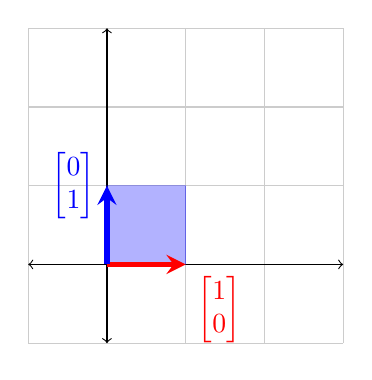
\begin{tikzpicture}[scale=1]
\draw[thin,gray!40] (-1,-1) grid (3,3);
  \draw[<->] (-1,0)--(3,0);
  \draw[<->] (0,-1)--(0,3);
  
  \filldraw[blue, opacity=0.3](0,0)--(1,0)--(1,1)--(0,1)--cycle;
  
\draw[line width=2pt,red,-stealth](0,0)--(1,0) node[below right]{$\begin{bmatrix}1\\0\end{bmatrix}$};

 \draw[line width=2pt,blue,-stealth](0,0)--(0,1) node[left]{$\begin{bmatrix}0\\1\end{bmatrix}$};
 
\end{tikzpicture}
\end{image}
We are used to working with column vectors.  In this section, however, when we use vectors to form a matrix we will regard them as row vectors.  So, the vector $\begin{bmatrix}1\\0\end{bmatrix}$ forms the first row, $\begin{bmatrix}1&0\end{bmatrix}$, of the matrix $\begin{bmatrix}1&0\\0&1\end{bmatrix}$.

If we double one of the vectors, the determinant doubles, and so does the area of the parallelogram.  
$$\begin{vmatrix}1&0\\0&2\end{vmatrix}=2\begin{vmatrix}1&0\\0&1\end{vmatrix}$$

\begin{image}[1.3in]
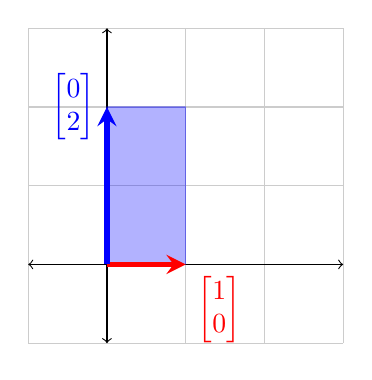
\begin{tikzpicture}[scale=1]
\draw[thin,gray!40] (-1,-1) grid (3,3);
  \draw[<->] (-1,0)--(3,0);
  \draw[<->] (0,-1)--(0,3);
  
  \filldraw[blue, opacity=0.3](0,0)--(1,0)--(1,2)--(0,2)--cycle;
  
\draw[line width=2pt,red,-stealth](0,0)--(1,0) node[below right]{$\begin{bmatrix}1\\0\end{bmatrix}$};

 \draw[line width=2pt,blue,-stealth](0,0)--(0,2) node[left]{$\begin{bmatrix}0\\2\end{bmatrix}$};
 
\end{tikzpicture}
\end{image}

If we shear the figure, the area is not affected (why?), but neither is the determinant.
$$\begin{vmatrix}1&0\\k&1\end{vmatrix}=1$$
(Note that we are using the two vectors as rows of the matrix.)
\begin{image}[1.3in]
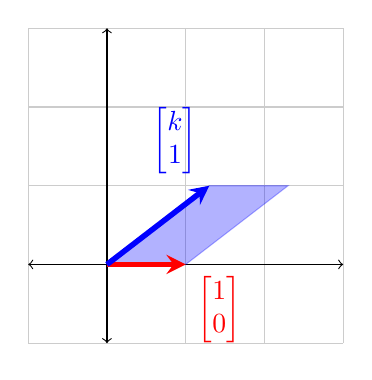
\begin{tikzpicture}[scale=1]
\draw[thin,gray!40] (-1,-1) grid (3,3);
  \draw[<->] (-1,0)--(3,0);
  \draw[<->] (0,-1)--(0,3);
  
  \filldraw[blue, opacity=0.3](0,0)--(1,0)--(2.3,1)--(1.3,1)--cycle;
  
\draw[line width=2pt,red,-stealth](0,0)--(1,0) node[below right]{$\begin{bmatrix}1\\0\end{bmatrix}$};

 \draw[line width=2pt,blue,-stealth](0,0)--(1.3,1) node[above left]{$\begin{bmatrix}k\\1\end{bmatrix}$};
 
\end{tikzpicture}
\end{image}

Three-by-three determinants can be interpreted as volumes in a similar way.  We will now proceed to derive the relationship between determinants, area and volume more formally.


\section*{$2\times 2$ Determinant and the Area of a Parallelogram}

Consider the parallelogram determined by vectors $\vec{u}$ and $\vec{v}$ in $\RR^3$.

\begin{image}[2.5in]
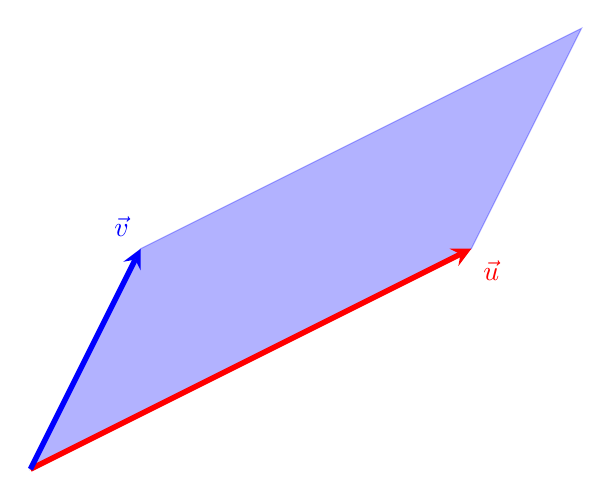
\begin{tikzpicture}[scale=1.4]

  \filldraw[blue, opacity=0.3](0,0)--(4,2)--(5,4)--(1,2)--cycle;

\draw[line width=2pt,red,-stealth](0,0)--(4,2) node[below right]{$\vec{u}$};
 
  \draw[line width=2pt,blue, -stealth](0,0)--(1,2) node[above left]{$\vec{v}$}; 
\end{tikzpicture}
\end{image}

Recall that the area of a parallelogram is given by the product of the length of the base and the height.
As shown in the diagram below, the length of the base is the magnitude of $\vec{u}$. The height, $h$, can be found using trigonometry $$h=\norm{\vec{v}}\sin\theta$$ 
\begin{image}[3in]
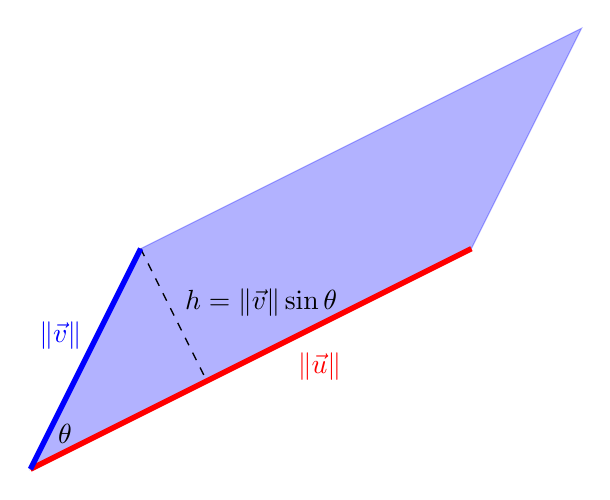
\begin{tikzpicture}[scale=1.4]

  \filldraw[blue, opacity=0.3](0,0)--(4,2)--(5,4)--(1,2)--cycle;

\draw[line width=0.5pt, dashed](1,2)--(1.6,0.8) node[above=1cm, right=-0.4cm]{$h=\norm{\vec{v}}\sin\theta$};

\draw[line width=2pt,red](0,0)--(4,2) node[below=1.5cm, left=1.5cm]{$\norm{\vec{u}}$};
 
  \draw[line width=2pt,blue](0,0)node[above=0.45cm, right=0.2cm, black]{$\theta$}--(1,2) node[below=1.1cm, left=0.6cm]{$\norm{\vec{v}}$}; 
\end{tikzpicture}
\end{image}
Using the area of a parallelogram formula together with Theorem \ref{th:crossproductsin} we get
$$\textnormal{Area}=(\text{base})(\text{height})=\norm{\vec{u}}h=\norm{\vec{u}}\norm{\vec{v}}\sin\theta=\norm{\vec{u}\times\vec{v}}$$
We have established the following formula.

\begin{formula}\label{form:areaofparallelogram} The area of a parallelogram determined by vectors $\vec{u}$ and $\vec{v}$ in $\RR^3$ is given by
$$\textnormal{Area}=\norm{\vec{u}\times\vec{v}}$$
\end{formula}

\begin{example}\label{ex:areaofparallelogram}
Find the area of the parallelogram in the diagram.
\begin{image}[3.5in]
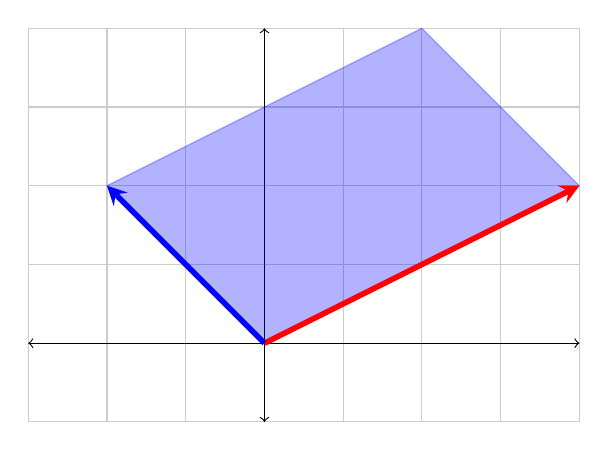
\begin{tikzpicture}[scale=1]
\draw[thin,gray!40] (-3,-1) grid (4,4);
  \draw[<->] (-3,0)--(4,0);
  \draw[<->] (0,-1)--(0,4);
  
  \filldraw[blue, opacity=0.3](0,0)--(-2,2)--(2,4)--(4,2)--cycle;

\draw[line width=2pt,red,-stealth](0,0)--(4,2);


 \draw[line width=2pt,blue,-stealth](0,0)--(-2,2);
 
\end{tikzpicture}
\end{image}
\begin{explanation}
The vectors that determine the parallelogram are 
$$\begin{bmatrix}4\\2\end{bmatrix}\quad\text{and}\quad\begin{bmatrix}-2\\2\end{bmatrix}$$
The problem we run into is that these vectors are in $\RR^2$, whereas the cross product is defined only for vectors in $\RR^3$.  We will get around this difficulty by ``padding" our vectors with zeros on the bottom.  In other words, we will consider them as vectors sitting in the $xy$-coordinate plane in $\RR^3$.  This allows us to compute the cross product 
$$\begin{bmatrix}4\\2\\0\end{bmatrix}\times\begin{bmatrix}-2\\2\\0\end{bmatrix}=\begin{vmatrix}\vec{i}&\vec{j}&\vec{k}\\4&2&0\\-2&2&0\end{vmatrix}=\vec{k}\Big((4)(2)-(2)(-2)\Big)=12\vec{k}=\begin{bmatrix}0\\0\\12\end{bmatrix}$$
The area of the parallelogram is then given by
$$\textnormal{Area}=\norm{\begin{bmatrix}0\\0\\12\end{bmatrix}}=12$$
\end{explanation}
\end{example}
\begin{general}
Example \ref{ex:areaofparallelogram} illustrates an important phenomenon.  Observe that the zeros in the last column of the determinant ensure that the $\vec{i}$ and $\vec{j}$ components of the cross product are zero, while the last component is the determinant of the $2\times 2$ matrix whose rows are the two vectors that determine the parallelogram in $\RR^2$.  In general, if the parallelogram is determined by vectors 
$$\begin{bmatrix}a\\b\end{bmatrix}\quad\text{and}\quad\begin{bmatrix}c\\d\end{bmatrix}$$
then the area of the parallelogram can be computed as follows:
$$\begin{bmatrix}a\\b\\0\end{bmatrix}\times\begin{bmatrix}c\\d\\0\end{bmatrix}=\begin{vmatrix}\vec{i}&\vec{j}&\vec{k}\\a&b&0\\c&d&0\end{vmatrix}=\vec{k}\begin{vmatrix}a&b\\c&d\end{vmatrix}=\vec{k}\Big((a)(d)-(b)(c)\Big)=\begin{bmatrix}0\\0\\ad-bc\end{bmatrix}$$

$$\textnormal{Area}=\norm{\begin{bmatrix}0\\0\\ad-bc\end{bmatrix}}=|ad-bc|=\Big|\det\begin{bmatrix}a&b\\c&d\end{bmatrix}\Big|$$

So the area of the parallelogram turns out to be the absolute value of the determinant of the matrix whose rows are the two vectors that determine the parallelogram. 
The following formula summarizes our discussion.
\begin{formula}\label{form:areaofparallelogramdeterminant} Let $\vec{u}=\begin{bmatrix}a\\b\end{bmatrix}$ and $\vec{v}=\begin{bmatrix}c\\d\end{bmatrix}$ be vectors of $\RR^2$.  The area of the parallelogram determined by $\vec{u}$ and $\vec{v}$ is given by
$$\textnormal{Area}=\Big|{\det\begin{bmatrix}a&b\\c&d\end{bmatrix}}\Big|$$
\end{formula}
\end{general}

\section*{$3\times 3$ Determinant and the Volume of a Parallelepiped}

Our next goal is to find the volume of a three-dimensional figure called a \dfn{parallelepiped}.  A parallelepiped is a six-faced figure whose opposite faces are congruent parallelograms located in parallel planes.  A parallelepiped is a three-dimensional counterpart of a parallelogram, and is determined by three non-coplanar vectors in $\RR^3$.  The figure below shows a parallelepiped determined by three vectors.

\begin{image}[4in]
\tdplotsetmaincoords{70}{130}
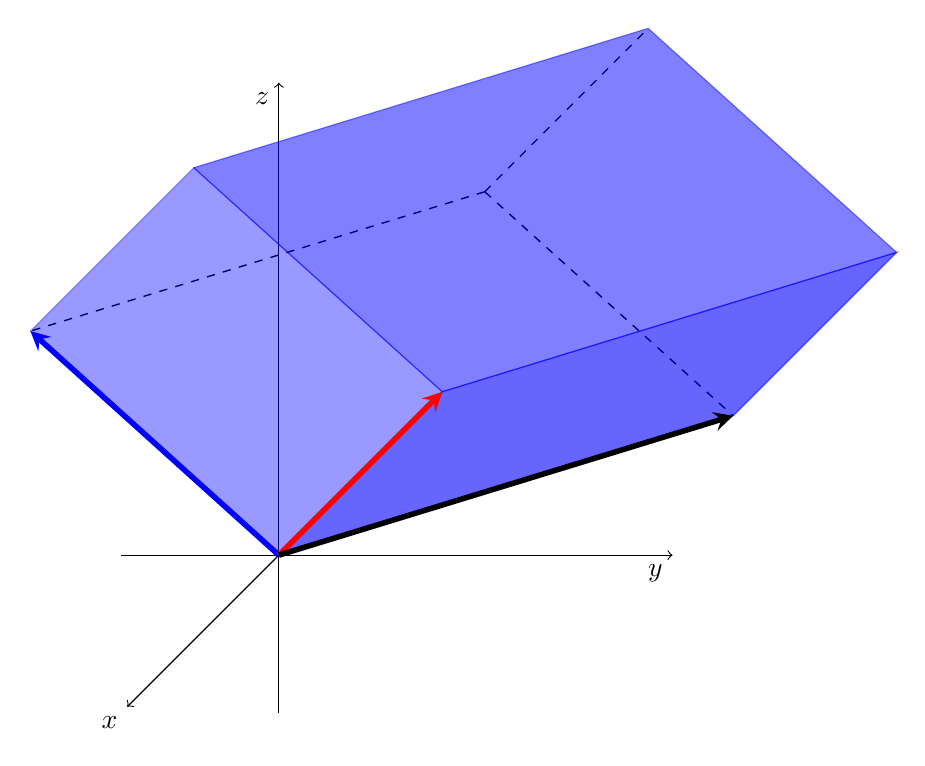
\begin{tikzpicture}
	\draw[->](-2,0,0)--(5,0,0) node[below left]{$y$};
    \draw[->](0,-2,0)--(0,6,0) node[below left]{$z$};
    \draw[->](0,0,-2)--(0,0,5) node[below left]{$x$};
    
    \draw[line width=0.5pt, dashed](3,5,1)--(5,1,-2);
    \draw[line width=0.5pt, dashed](3,5,1)--(-2,4,3);
    \draw[line width=0.5pt, dashed](3,5,1)--(7,9,6);
    
  %  \draw[line width=0.5pt, dashed](9,5,3)--(131/16,113/16,2);
    
    \filldraw[blue, opacity=0.4] (0,0,0)--(-2, 4, 3)--(2,8,8)--(4,4,5)--cycle;
    \filldraw[blue, opacity=0.5] (2,8,8)--(4,4,5)--(9,5,3)--(7,9,6)--cycle;
    \filldraw[blue, opacity=0.6] (0,0,0)--(4,4,5)--(9,5,3)--(5,1,-2)--cycle;
    
    \draw[->, line width=2pt,blue, -stealth](0,0,0)--(-2,4,3);
    \draw[->, line width=2pt,red, -stealth](0,0,0)--(4,4,5);
    \draw[->, line width=2pt, -stealth](0,0,0)--(5,1,-2);
    
\end{tikzpicture}
\end{image}

Consider a parallelepiped determined by vectors $\vec{u}$, $\vec{v}$ and $\vec{w}$, as shown below.  

\begin{image}
\tdplotsetmaincoords{70}{130}
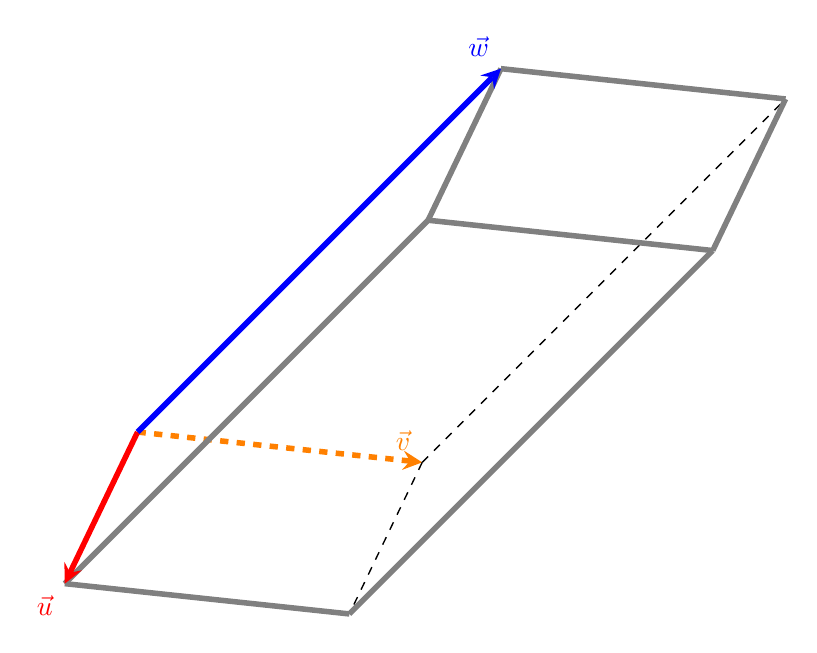
\begin{tikzpicture}
    \draw[->, line width=2pt, -stealth,orange,dashed](0,0,0)--(4,0,1)node[above left]{$\vec{v}$};
    
    \draw[line width=0.5pt, dashed](4,0,1)--(5,0,6);
    \draw[line width=0.5pt, dashed](4,0,1)--(9,5,2);
    
    %\draw[line width=0.5pt, dashed](5,5,1)--(0,5,0);
    
    \draw[line width=2pt, gray](1,0,5)--(6,5,6);
    \draw[line width=2pt, gray](10,5,7)--(6,5,6);
    \draw[line width=2pt, gray](10,5,7)--(5,0,6);
    \draw[line width=2pt, gray](1,0,5)--(5,0,6);
    \draw[line width=2pt, gray](6,5,6)--(5,5,1);
    \draw[line width=2pt, gray](9,5,2)--(5,5,1);
    \draw[line width=2pt, gray](10,5,7)--(9,5,2);
    
    \draw[->, line width=2pt,red, -stealth](0,0,0)--(1,0,5)node[below left]{$\vec{u}$};
    \draw[->, line width=2pt, blue, -stealth](0,0,0)--(5,5,1)node[above left]{$\vec{w}$} ;
    
   % \draw[->, line width=1pt, -stealth](0,0,0)--(0,6,0) node[above]{$\vec{u}\times\vec{v}$};
    %\draw[->, gray, line width=0.5pt, -stealth](-0.25,2.5,0)node[left, black]{$h$}--(-0.25,0,0);
    %\draw[->, gray, line width=0.5pt, -stealth](-0.25,2.5,0)--(-0.25,5,0);
\end{tikzpicture}
\end{image}

The volume of a parallelepiped is given by 
$$\textnormal{Volume}=(\text{area of base})(\text{height})$$
We will consider the parallelogram determined by $\vec{u}$ and $\vec{v}$ to be the base of the parallelepiped.  Thus, the area of the base is given by 
$$\textnormal{Area of Base}=\norm{\vec{u}\times\vec{v}}$$
\begin{image}
\tdplotsetmaincoords{70}{130}
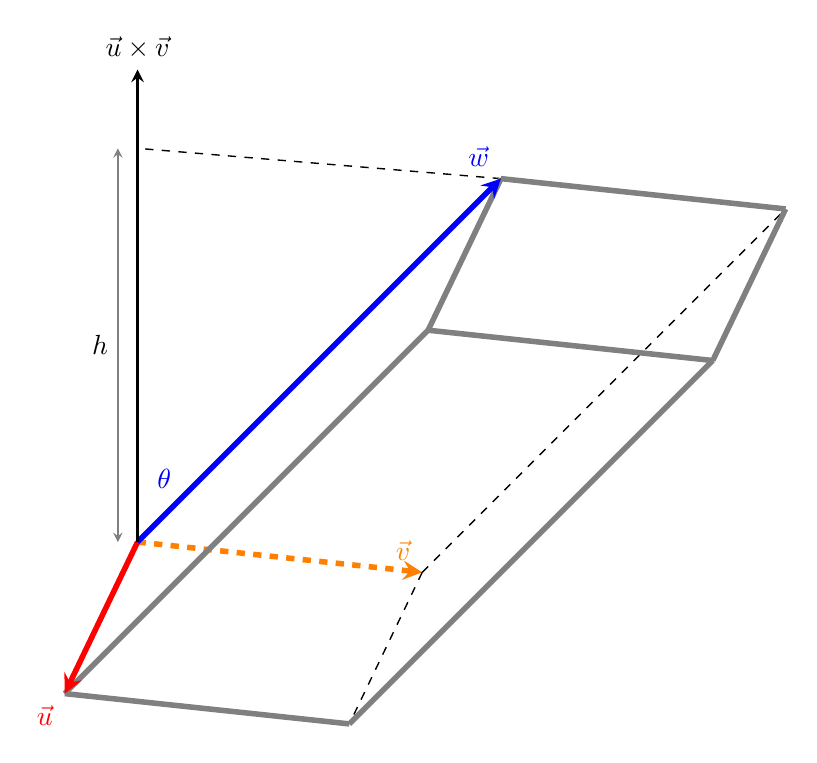
\begin{tikzpicture}
    \draw[->, line width=2pt, -stealth,orange,dashed](0,0,0)--(4,0,1)node[above left]{$\vec{v}$};
    
    \draw[line width=0.5pt, dashed](4,0,1)--(5,0,6);
    \draw[line width=0.5pt, dashed](4,0,1)--(9,5,2);
    
    \draw[line width=0.5pt, dashed](5,5,1)--(0,5,0);
    
    \draw[line width=2pt, gray](1,0,5)--(6,5,6);
    \draw[line width=2pt, gray](10,5,7)--(6,5,6);
    \draw[line width=2pt, gray](10,5,7)--(5,0,6);
    \draw[line width=2pt, gray](1,0,5)--(5,0,6);
    \draw[line width=2pt, gray](6,5,6)--(5,5,1);
    \draw[line width=2pt, gray](9,5,2)--(5,5,1);
    \draw[line width=2pt, gray](10,5,7)--(9,5,2);
    
    \draw[->, line width=2pt,red, -stealth](0,0,0)--(1,0,5)node[below left]{$\vec{u}$};
    \draw[->, line width=2pt, blue, -stealth](0,0,0)node[above=0.8cm, right=0.1cm]{$\theta$}--(5,5,1)node[above left]{$\vec{w}$} ;
    
    \draw[->, line width=1pt, -stealth](0,0,0)--(0,6,0) node[above]{$\vec{u}\times\vec{v}$};
    \draw[->, gray, line width=0.5pt, -stealth](-0.25,2.5,0)node[left, black]{$h$}--(-0.25,0,0);
    \draw[->, gray, line width=0.5pt, -stealth](-0.25,2.5,0)--(-0.25,5,0);
\end{tikzpicture}
\end{image}

The height of the parallelepiped is measured along a line perpendicular to the base.  By Theorem \ref{th:crossproductorthtouandv}, $\vec{u}\times\vec{v}$ lies on such a line.  Let $\theta$ be the angle between $\vec{w}$ and $\vec{u}\times\vec{v}$, $0\leq \theta\leq\pi$.  Then the height, $h$, of the parallelepiped is given by 
$$h=\norm{\vec{w}}|\cos\theta |$$
This gives us the following formula for the volume of the parallelepiped
$$\textnormal{Volume}=\norm{\vec{u}\times\vec{v}}\norm{\vec{w}}|\cos\theta |=|(\vec{u}\times\vec{v})\dotp\vec{w}|$$

We have established the following formula.
\begin{formula}
The volume of a parallelepiped determined by vectors $\vec{u}$, $\vec{v}$ and $\vec{w}$ in $\RR^3$ is given by\\
$$\textnormal{Volume}=|(\vec{u}\times\vec{v})\dotp\vec{w}|$$
\end{formula}

Our next goal is to show that this expression for the volume is equal to the determinant of a $3\times 3$ matrix whose rows are the vectors that determine the parallelepiped.

Let 
$$\vec{u}=\begin{bmatrix}u_1\\u_2\\u_3\end{bmatrix},\quad\vec{v}=\begin{bmatrix}v_1\\v_2\\v_3\end{bmatrix},\quad\vec{w}=\begin{bmatrix}w_1\\w_2\\w_3\end{bmatrix}$$
then
\begin{align}\label{eq:boxproduct}(\vec{u}\times\vec{v})\dotp\vec{w}=\begin{vmatrix}\vec{i}&\vec{j}&\vec{k}\\u_1&u_2&u_3\\v_1&v_2&v_3\end{vmatrix}\dotp\begin{bmatrix}w_1\\w_2\\w_3\end{bmatrix}=\begin{vmatrix}w_1&w_2&w_3\\u_1&u_2&u_3\\v_1&v_2&v_3\end{vmatrix}
\end{align}
The expression in (\ref{eq:boxproduct}) is sometimes referred to as the \dfn{box product}.

\begin{formula}
Let $\vec{u}=\begin{bmatrix}u_1\\u_2\\u_3\end{bmatrix},\quad\vec{v}=\begin{bmatrix}v_1\\v_2\\v_3\end{bmatrix},\quad\vec{w}=\begin{bmatrix}w_1\\w_2\\w_3\end{bmatrix}$ be vectors in $\RR^3$.  Then the volume of the parallelepiped determined by $\vec{u}$, $\vec{v}$ and $\vec{w}$ is given by 
$$\textnormal{Volume}=\Big|\det\begin{bmatrix}w_1&w_2&w_3\\u_1&u_2&u_3\\v_1&v_2&v_3\end{bmatrix}\Big|$$
\end{formula}

\section*{Practice Problems}

\begin{problem} Let $S$ be a square determined by $\begin{bmatrix}2\\0\end{bmatrix}$ and $\begin{bmatrix}0\\2\end{bmatrix}$.  Let $P$ be a parallelogram determined by vectors $\begin{bmatrix}2\\5\end{bmatrix}$ and $\begin{bmatrix}0\\2\end{bmatrix}$.  Sketch both figures in the same coordinate plane, and use geometry to explain why $S$ and $P$ have the same area.  Compute the area of $P$ using Formula \ref{form:areaofparallelogramdeterminant}.

Answer: $$\text{Area of }P=\answer{4}$$
\end{problem}

\begin{problem}
Supply the intermediate steps in (\ref{eq:boxproduct}).
\end{problem}

\begin{problem}
Find the volume of a parallelepiped determined by 
$$\begin{bmatrix}0\\5\\4\end{bmatrix}\quad\begin{bmatrix}3\\1\\2\end{bmatrix}\quad\begin{bmatrix}1\\1\\6\end{bmatrix}$$
Answer: $\textnormal{Volume}=\answer{72}$
\end{problem}

\begin{problem}
Find the volume of a parallelepiped determined by 
$$\begin{bmatrix}1\\4\\-1\end{bmatrix}\quad\begin{bmatrix}3\\-2\\4\end{bmatrix}\quad\begin{bmatrix}5\\6\\2\end{bmatrix}$$
Explain your result geometrically.

Answer: $\textnormal{Volume}=\answer{0}$
\end{problem}


\end{document} 
